\section{Overview of ILC and SaUCy}
\label{sec:background}

We tour the universal composability framework and give a flavor of ILC and SaUCy
with the simple example of how two untrusting parties, Alice and Bob, can
securely flip a coin using a commitment scheme.

\begin{figure*}[t]
\centering
\begin{tabular}{c|c}
\begin{subfigure}{.575\textwidth}
    $\Func_{\textsc{com}}$ proceeds as follows, running with parties $A$ and
  $B$.
    \begin{enumerate}
        \item Upon receiving a message $(\mathsf{Commit}, b)$ from $A$, where $b
          \in \{ 0, 1 \}$, record the value $b$ and send the message
          $(\mathsf{Receipt})$ to $B$. Ignore any subsequent \textsf{Commit}
          messages.
        \item Upon receiving a message $(\mathsf{Open})$ from $A$, proceed as
          follows: If some value $b$ was previously recorded, then send the
          message $(\mathsf{Open}, b)$ to $B$ and halt. Otherwise, halt.
    \end{enumerate}
\label{func:com}
\end{subfigure}\hspace{0.02\textwidth}
&\hspace{0.02\textwidth}
\begin{subfigure}{.35\textwidth}
  \lstinputlisting[style=myilc]{listings/Fcom.ilc}
\end{subfigure}
\end{tabular}
\caption{An ideal functionality for a one-time commitment scheme in prose (left)
  and in ILC (right).}
\label{func:com}
\end{figure*}

\subsection{Ideal Functionalities}
\label{subsec:functionalities}

Security in the UC framework is based on the real/ideal
paradigm~\cite{goldreich1987play}. To carry out some cryptographic task in the
real world, a set of parties must execute a protocol for the task among
themselves in a distributed fashion. In the ideal world, however, the parties
securely access an \emph{ideal functionality} $\mc{F}$, which is imagined as an
incorruptible trusted third party that securely (by construction) carries out
the task to be achieved by the protocol. The idea is that $\mc{F}$ obtains
inputs from the parties, carries out the task locally, and returns outputs back
to the parties. This serves as a self-contained specification
for the task's security requirements.\smallskip

\myheader{Example: Secure coin flipping.} Suppose two untrusting parties, Alice
and Bob, wish to securely flip a coin---Alice calls the coin flip by publishing $b
\in \{ 0, 1\}$, and Bob flips the coin by publishing $r \in \{0, 1\}$. If $b = r$,
then Alice wins; otherwise, Bob wins. Observe that simply having Alice and Bob
publish their respective values is not secure. If Alice publishes $b$ first,
then Bob can cheat by manipulating $r$ in his favor (and vice versa)!

In order to carry out the coin flip securely, they can use a commitment
scheme~\cite{brassard1988minimum}. Alice first publishes a commitment $C =
\mathsf{com}(b)$ for her bit $b$, waits for Bob to publish $r$, and then opens
and publishes a bit $b' = \mathsf{open}(C)$. If $r = b'$, then Alice wins;
otherwise, Bob wins.  Now, in order for such a commitment scheme to be secure,
it should satisfy the \emph{hiding} property (i.e., $C$ hides $b$ from Bob, so
he cannot manipulate $r$ in his favor) and the \emph{binding} property (i.e.,
$b=b'$, so that Alice cannot change the committed value in her favor).\smallskip

\myheader{Commitment functionality.} We can capture both of these properties at
once by defining an ideal functionality $\Func_{\textsc{com}}$ for a (one-time)
commitment scheme as it would appear in the cryptography literature
(Figure~\ref{func:com}, left). Upon receiving the bit $b$ that Alice commits to,
$\Func_{\textsc{com}}$ records $b$ and notifies Bob that it has done so. Then,
whenever Alice wants to reveal $b$ to Bob, she notifies $\Func_{\textsc{com}}$,
which sends it to Bob. Because, in this idealized world, Alice and Bob trust
$\Func_{\textsc{com}}$ to do all the work, the hiding and binding properties
hold trivially. Of course, in the real world, Alice and Bob would not want to
trust such a third party (if it even exists), so their hope is that the
commitment scheme they use is ``just as good as''
$\Func_{\textsc{com}}$.\smallskip

\myheader{Commitment functionality in ILC.} In Figure~\ref{func:com} (right), we
have written $\Func_{\textsc{com}}$ in ILC. The function \textsf{fCom} takes as
arguments a read channel \textsf{frA}, which receives messages from $A$, and a
write channel \textsf{toB}, which sends messages to $B$. In ILC, channels are
typed, so each of these channels communicates values inhabiting the sum type
\textsf{Msg}. Moreover, read channels are linearly typed so that they are
protected from duplication. This ensures that no confusion arises as to which
process is being written to. On the other hand, write channels are
intuitionistically typed, so their use is unrestricted.

Because \textsf{fCom} consumes a linear read channel, its type signature
consists of linear arrows $\lolli$ (or ``lollipops''), which describe the types
of linear functions that consume their arguments exactly once. But what if a
linear function wishes to consume an intuitionistically typed argument? In that
case, the ! operator (pronounced ``bang!'') permits an intuitionistically typed
value to be used in an unrestricted manner as a linearly typed value, i.e.,
contraction or weakening may be used. This explains why the type of \textsf{frA}
is \textsf{Rd Msg} and the type of \textsf{toB} is \textsf{!(Wr Msg)}.

ILC expressions are also typed with a mode $m \in \{\Wm, \Rm, \Vm\}$, denoting
write, read, and value modes, respectively. Arrow types, both linear and
intuitionistic, carry the mode of their function bodies, so in the function
signature for \textsf{fCom}, the left lollipop implicitly carries a mode $\Vm$,
which we have chosen to elide, and the right lollipop carries a mode $\Rm$,
which is the mode of its body. The function body of \textsf{fCom} closely
follows $\Func_{\textsc{com}}$, but several points are worth mentioning.

First, we introduce the typing rules of expressions for reading and writing on a
channel. Recall that typing judgements have the form $\Delta ; \Gamma |- e : A |> m$,
where $\Delta$ is a linear typing context and $m \in \{\Wm, \Rm, \Vm\}$ is a mode.
\begin{mathpar}
\Infer{letrd}
{\Delta_1 ; \Gamma |- e_1 : \tyRd{A}\\
\Delta_2,x_1:\tyBang{A},x_2:\tyRd{A} ; \Gamma |- e_2 : B |> m
}
{\Delta_1, \Delta_2 ; \Gamma |- \eLetRd{x_1}{x_2}{e_1}{e_2} : B |> \Rm}
\end{mathpar}

The letrd rule says that if we can partition the linear context $\Delta$ as $\Delta_1,
\Delta_2$ such that $e_1$ has type $\tyRd{A}$ and mode $\Vm$ (elided) under contexts
$\Delta_1, \Gamma$ and $e_2$ has type $B$ and mode $m$ under contexts
$\Delta_2,x_1:\tyBang{A},x_2:\tyRd{A} ; \Gamma$, then the full expression has type $B$ and
mode $\Rm$. Here, the idea is that reading a channel of type $\tyRd{A}$ gives a
linear pair (or ``tensor'') of type $\tyTensor{\tyBang{A}}{\tyRd{A}}$. Because
only intuitionistically typed values can be sent over channels in ILC, the first
element of the tensor lifts the value read from the channel into a linear type,
and the second element rebinds the read channel, so that it may be used again.
In \textsf{fCom}, pattern matching with the ! operator unpacks linearly typed
values, so the value bound to the $b$ in the first read from \textsf{frA} has an
intuitionistic type.
\begin{mathpar}
\Infer{wr}
{\Delta_1; \Gamma   |- e_1 : A\\
\Delta_2; \Gamma   |- e_2 : \tyWr{A}}
{\Delta_1, \Delta_2; \Gamma |- \eWr{e_1}{e_2} : \tyUnit |> \Wm}
\end{mathpar}

The wr rule says that if we can partition the linear context $\Delta$ as $\Delta_1, \Delta_2$
such that $e_1$ has type $A$ and mode $\Vm$ and $e_2$ has a type $\tyWr{A}$ and
mode $\Vm$, then the full expression has type $\tyUnit$ and mode $\Wm$.

What is not showcased in these two rules is mode composition. In ILC, modes can
be composed in two ways: sequentially (i.e., $m ;; n => p$) and in parallel
(i.e., $m || n => p$). The rules for mode composition, which we describe in full
in Section~\ref{sec:ilc}, prevent composing two write mode processes in
parallel. That is, $\Wm || \Wm => p$ is not derivable for any mode $p$. This
ensures that no confusion arises as to which process is writing and hence,
activated, since in the ITM model only a single process is active at any given
time. In \textsf{fCom}, each of the letrd expressions is read mode, and
sequentially composing two read mode expressions yields a read mode expression
(i.e., $\Rm ;; \Rm => \Rm$ according to our mode composition rules). As
aforementioned, the right lollipop in \textsf{fCom}'s type signature carries the
mode $\Rm$.

\subsection{UC Emulation}
\label{subsec:emulation}

We say that a protocol $\pi$ \emph{emulates} (or \emph{securely realizes})
$\mc{F}$ if any attack that is possible on $\pi$ is also possible on
$\mc{F}$. However, since $\mc{F}$ is designed to be secure by definition, such
an attack does not lead to a break in security.

Proving emulation formally proceeds in two steps. The first step is
constructive: We must construct a \emph{simulator} $\mc{S}$ (a simulated
adversary) that can emulate the attack of any adversary $\mc{A}$ on $\pi$, but
instead, on $\mc{F}$. The second step is a relational analysis: We must show
that running $\pi$ under attack by any adversary $\mc{A}$ (the real world) is
\emph{indistinguishable} from running $\mc{F}$ under attack by $\mc{S}$ (the
ideal world) to any distinguisher $\mc{Z}$, called the \emph{environment}. In
particular, $\mc{Z}$ is an interactive distinguisher: It interacts with the real
world and the ideal world in a well-defined manner, and the simulation is good
if no $\mc{Z}$ can distinguish between the two.

\begin{figure}
  \centering
  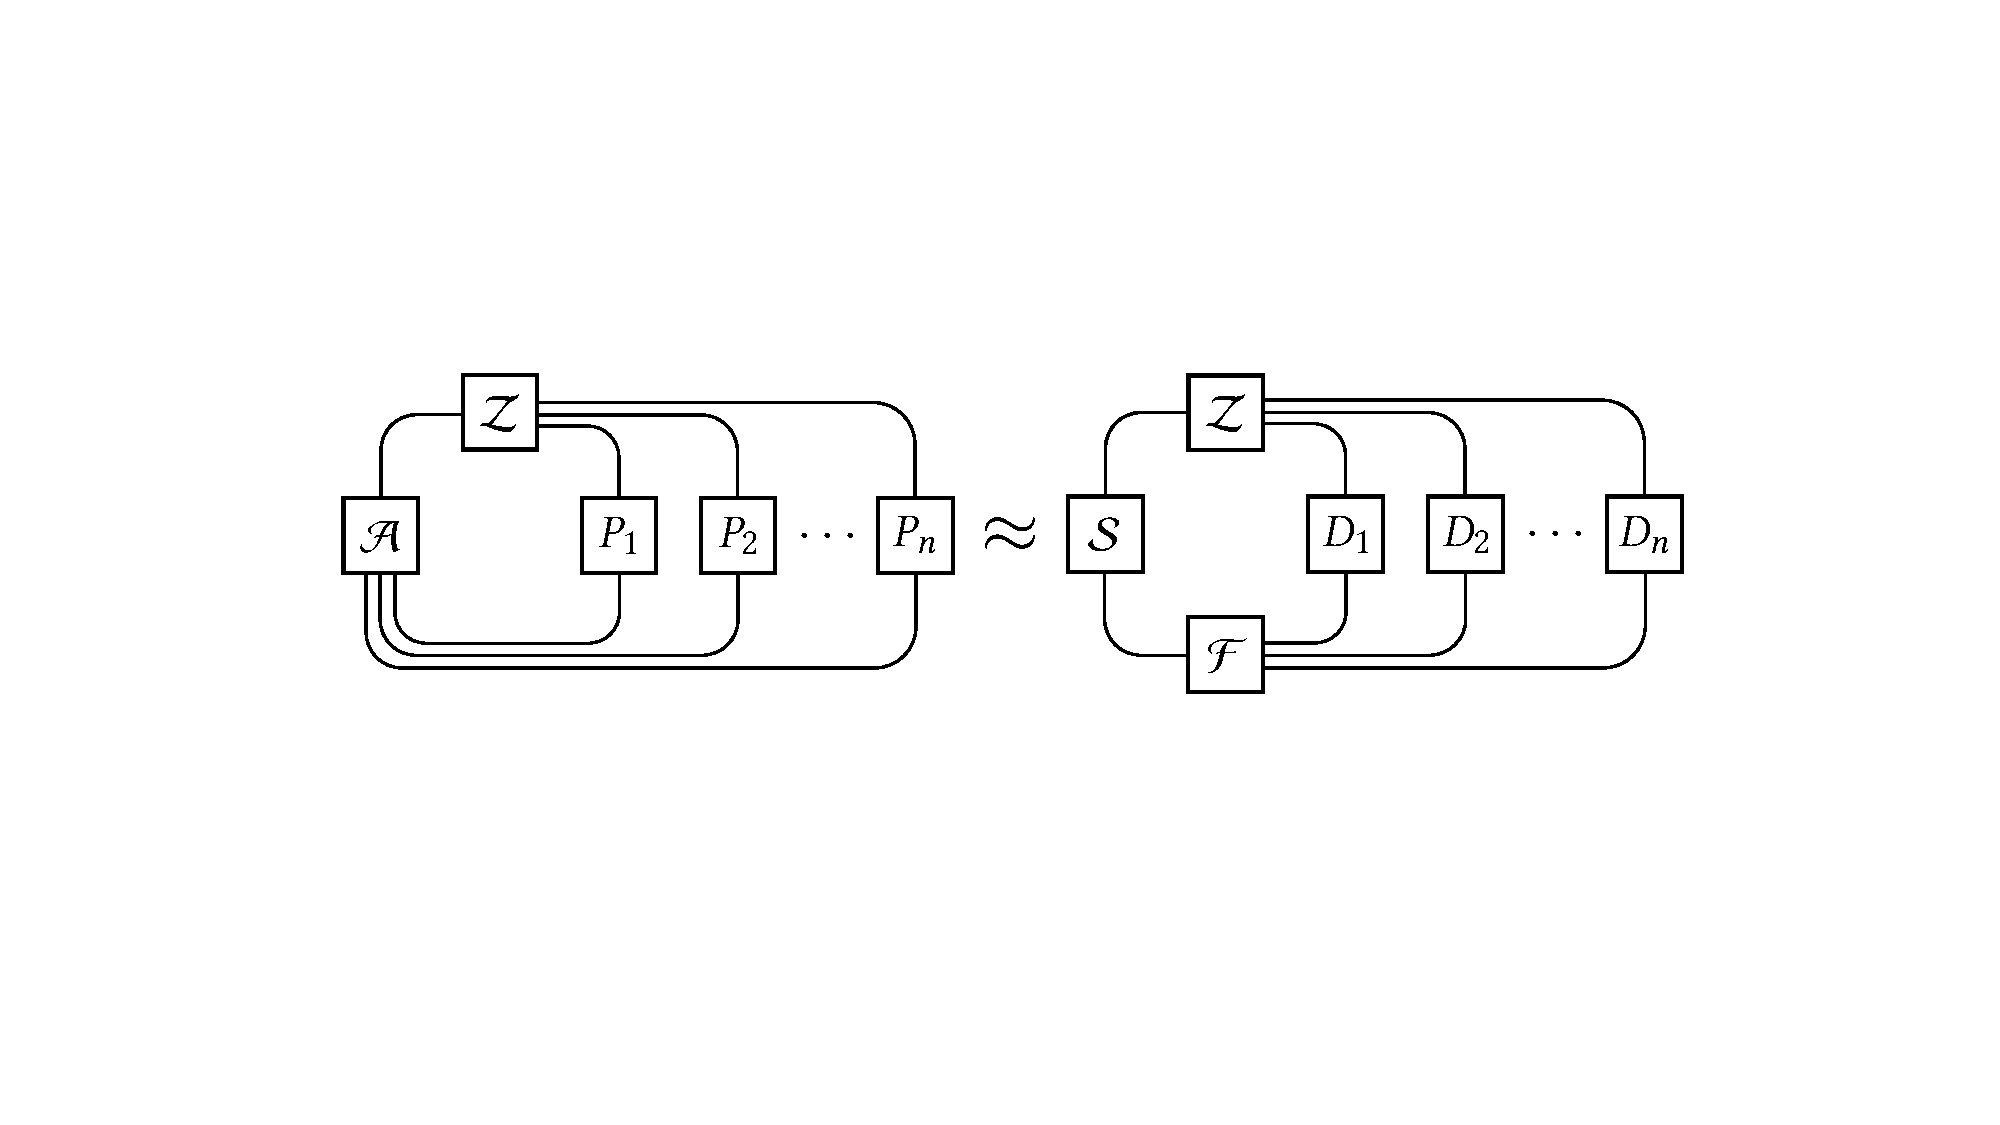
\includegraphics[width=\linewidth]{graphics/uc-experiment}
  \caption{UC experiment with real world (left) and ideal world (right).}
  \label{fig:uc-experiment}
\end{figure}

Figure~\ref{fig:uc-experiment} illustrates the UC experiment: connecting lines
denote communication channels,\footnote{Note that all communication passes
  through the adversary $\mc{A}$. In the bare model, communication is
  asynchronous, unauthenticated, and unreliable, but other models of
  communication can be built atop this model.} $P_1, P_2, \ldots, P_n$ represent
parties executing protocol $\pi$, and $D_1, D_2, \ldots, D_n$ represent ``dummy''
parties that simply relay information between the environment and the ideal
functionality.

\begin{comment}
\subsection{UC composition}
\label{subsec:composition}

The advantage of security definitions in UC is that they satisfy strong
composability guarantees, even under concurrent composition. Suppose that $\pi_1$
is a protocol that securely realizes a functionality $\mc{F}_1$. If a protocol
$\pi_2$, using $\mc{F}_1$ as a subroutine, securely realizes a functionality
$\mc{F}_2$, then the protocol $[\pi_1 / \mc{F}_1]\pi_2$, in which calls to
$\mc{F}_1$ are replaced by calls to $\pi_1$, also securely realizes
$\mc{F}_2$. That way, it suffices to analyze the security of the standalone
protocol $\pi_2$ in the $\mc{F}_1$-hybrid model, where parties run $\pi_2$ with
access to $\mc{F}_1$, as opposed to the composite protocol of $\pi_2$ and
$\pi_1$. Figure~\ref{fig:uc-composition} illustrates protocol composition. The
setup on the left represents the $\mc{F}_1$-hybrid model, and the setup on the
right represents the protocol substitution $[\pi_1 / \mc{F}_1]\pi_2$, which
maintains security.

\begin{figure}
  \centering
  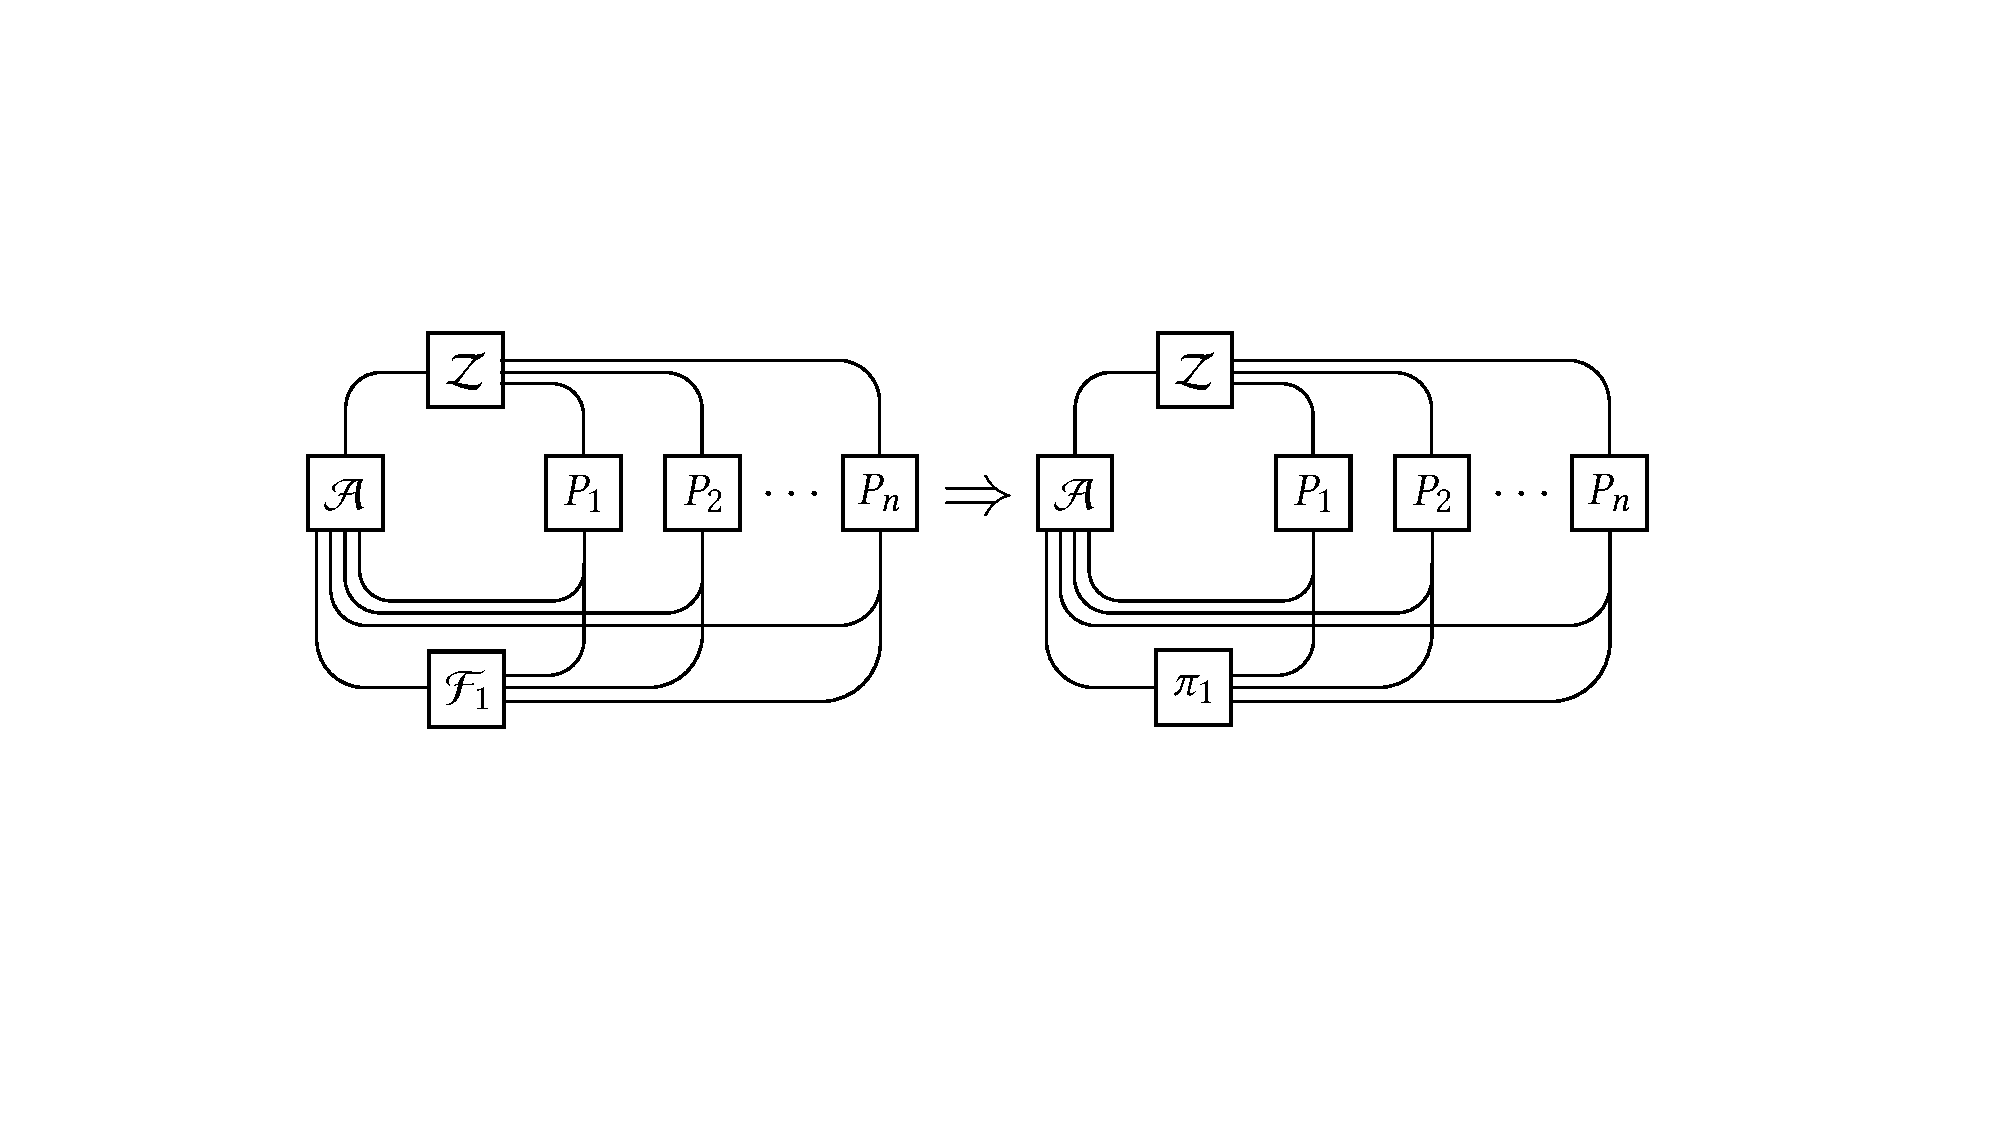
\includegraphics[width=\linewidth]{graphics/composition}
  \caption{UC protocol composition theorem.}
  \label{fig:uc-composition}
\end{figure}
\end{comment}
